\documentclass{article}
\usepackage[T1]{fontenc}
\usepackage{titlesec}
\usepackage{graphicx}
\usepackage{amsmath}
\usepackage{xcolor}
\usepackage{circuitikz}
\titleformat{\section}  % which section command to format
  {\fontsize{10}{12}\bfseries} % format for whole line
  {\thesection} % how to show number
  {1em} % space between number and text
  {} % formatting for just the text
  [] % formatting for after the text
\title{Logika Cyfrowa}
\author{Jakub Gałaszewski} 
\begin{document}
\maketitle
\section{Udowodnij, że sumator pełny zbudowany z półsumatorów zaprezentowany na wykładzie jest równoważny sumatorowi pełnemu skonstruowanemu za pomocą mapy Karnaugh.}
 \textbf{Półsumator} to układ złożony z dwóch bitów $a$ i $b$, a wyjściem jest $s$ i $c$ (odpowiednio suma i przeniesienie).\\
\textbf{Sumator} to układ złożony z trzech bitów $a$ i $b$ i $c$ (gdzie $c$ to potencjalne przeniesienie z poprzedniego równania), a wyjściem jest $s$ i $c_0$ (odpowiednio suma i przeniesienie).\\
Sumator przedstawiony na wykładzie to:
\begin{center}
\includegraphics[scale=0.5]{./L03Z01.png}

\includegraphics[scale=0.5]{./L03Z01czII.png}
\end{center}
Natomiast sumator za pomocą tabelki wygląda następująco:\\
	\begin{tabular}{|c|c|c||c|c|} 
	 \hline
	$a$ & $b$ & $c$ & $c_0$ & $s$\\ 
	 \hline \hline
	 0&0&0&0&0\\ \hline
	 0&0&1&0&1\\ \hline
	 0&1&0&0&1\\ \hline
	 0&1&1&1&0\\ \hline
	 1&0&0&0&1\\ \hline	 
	 1&0&1&1&0\\ \hline
	 1&1&0&1&0\\ \hline
	 1&1&1&1&1\\ \hline
	\end{tabular}
	%$c_0$\\
	\begin{tabular}{|c|c|c|c|c|} 
	$c_0$\\
	 \hline
	a\textbackslash bc& 00 & 01 & 11 & 10\\ 
	 \hline
	 0&0&0&1&0\\ \hline
	 1&0&1&1&1\\ \hline
	\end{tabular}
	%$s$\\
	\begin{tabular}{|c|c|c|c|c|} 
	$s$\\
	 \hline
	a\textbackslash bc& 00 & 01 & 11 & 10\\ 
	 \hline
	 0&0&1&0&1\\ \hline
	 1&1&0&1&0\\ \hline
	\end{tabular}\\
	\begin{center}
	$c_0=bc+ab+ac$\\ 
	$s=a\bar{b}\bar{c} + \bar{a}\bar{b}c + abc + \bar{a}b\bar{c}$
	\end{center}
	\begin{circuitikz} \draw
	(0,0)
	node [label=left:$c$]{}
	|-
	(2,0)
	node [and port, anchor=in 1] (andac) {}
	(0,0 |- andac.in 2)
	node [label=left:$a$]{}
	|-
	(andac.in 2)
	(2,-1.5)
	node [and port, anchor=in 1] (andab) {}
	(0,0 |- andab.in 1)
	node [label=left:$b$]{}
	|-
	(andab.in 1)
	(andab.in 2)
	-- ++(-0.25, 0)
	to[short, -*](1.75,0 |- andac.in 2)
	(2, -3)
	node [and port, anchor=in 1] (andbc) {}
	(andbc.in 1)
	-- ++(-0.5, 0)
	to[short, -*](1.5,0 |- andab.in 1)
	(andbc.in 2)
	-- ++(-0.75, 0)
	to[short, -*](1.25,0 |- andac.in 1)
	(5, 0 |- andab.out)
	node [or port, number inputs = 3, anchor = in 2] (or) {}
	(andbc.out) |- (or.in 3)
	(andac.out) |- (or.in 1)
	(andab.out) |- (or.in 2)	
	(or.out) 
	to[short, -] ++(1, 0) 
	node [label=right:$c_0$]	{}
	;
\end{circuitikz}\\
\begin{circuitikz} \draw
	(0,0)
	node [label=left:$c$]{}
	|-
	(2,0)
	node [not port, anchor=in] (notc) {}
	
	(0,-1.5)
	node [label=left:$a$]{}
	|-
	++(2,0)
	node [not port, anchor=in] (nota) {}
	
	(0,-3)
	node [label=left:$b$]{}
	|-
	++(2,0)
	node [not port, anchor=in] (notb) {}
	
	(notc.out)
	++(1,0)
	node [and port, number inputs = 3, anchor = in 1] (anbnc) {}
	
	(notc.out) -| (anbnc.in 1)
	(anbnc.in 2) -| (nota.out)
	(anbnc.in 3)
	to[short, -] ++ (-0.25, 0)
	to[short, -] ++ (0, -3)
	to[short, -] ++ (-2.15, 0)
	to[short, -*] (notb.in)
	
	(anbnc.in 2)
	++(0, -1.5)
	node [and port, number inputs = 3, anchor = in 1] (nanbc) {}
	(nota.out) |- (nanbc.in 1)
	(notb.out) |- (nanbc.in 2)
	(nanbc.in 3)
	to[short, -] ++ (-0.5, 0)
	to[short, -] ++ (0, -3)
	to[short, -] ++ (-2, 0)
	to[short, -*] (1.9, |- notc.in)
	
	(nanbc.in 2)
	++(0, -1.5)
	node [and port, number inputs = 3, anchor = in 1] (abc) {}
	(abc.in 3)
	to[short, -] ++ (0, -1)
	to[short, -] ++ (-2.7, 0)
	to[short, -*] (1.7, |- notb.in)
	(abc.in 2)
	to[short, -] ++ (-0.1, 0)	
	to[short, -] ++ (0, -1)
	to[short, -] ++ (-2.8, 0)
	to[short, -*] (1.5, |- nota.in)
	(abc.in 1)
	to[short, -] ++ (0, -1)
	to[short, -] ++ (-3.1, 0)
	to[short, -*] (1.3, |- notc.in)
	
	(abc.in 2)
	++(0, -1.5)
	node [and port, number inputs = 3, anchor = in 1] (nabnc) {}
	(nabnc.in 1) 
	to[short, -] ++(-0.4, 0)
	|- (nota.out)
	(nabnc.in 2) 
	to[short, -] ++(-0.6, 0)
	|- (notc.out)
	(nabnc.in 3)
	to[short, -] ++ (-2.7, 0)
	to[short, -*] (1.7, |- notb.in)
	
	(nanbc.in 2)
	++(4, -1)
	node [or port, number inputs = 4] (or) {}
	(anbnc.out) |- (or.in 1)
	(nanbc.out) |- (or.in 2)
	(abc.out) |- (or.in 3)	
	(nabnc.out) |- (or.in 4)
	(or.out)
	%to[short, -] ++(1, 0) 
	node [label=right:$s$]	{}
	;
\end{circuitikz}\\
\begin{center}
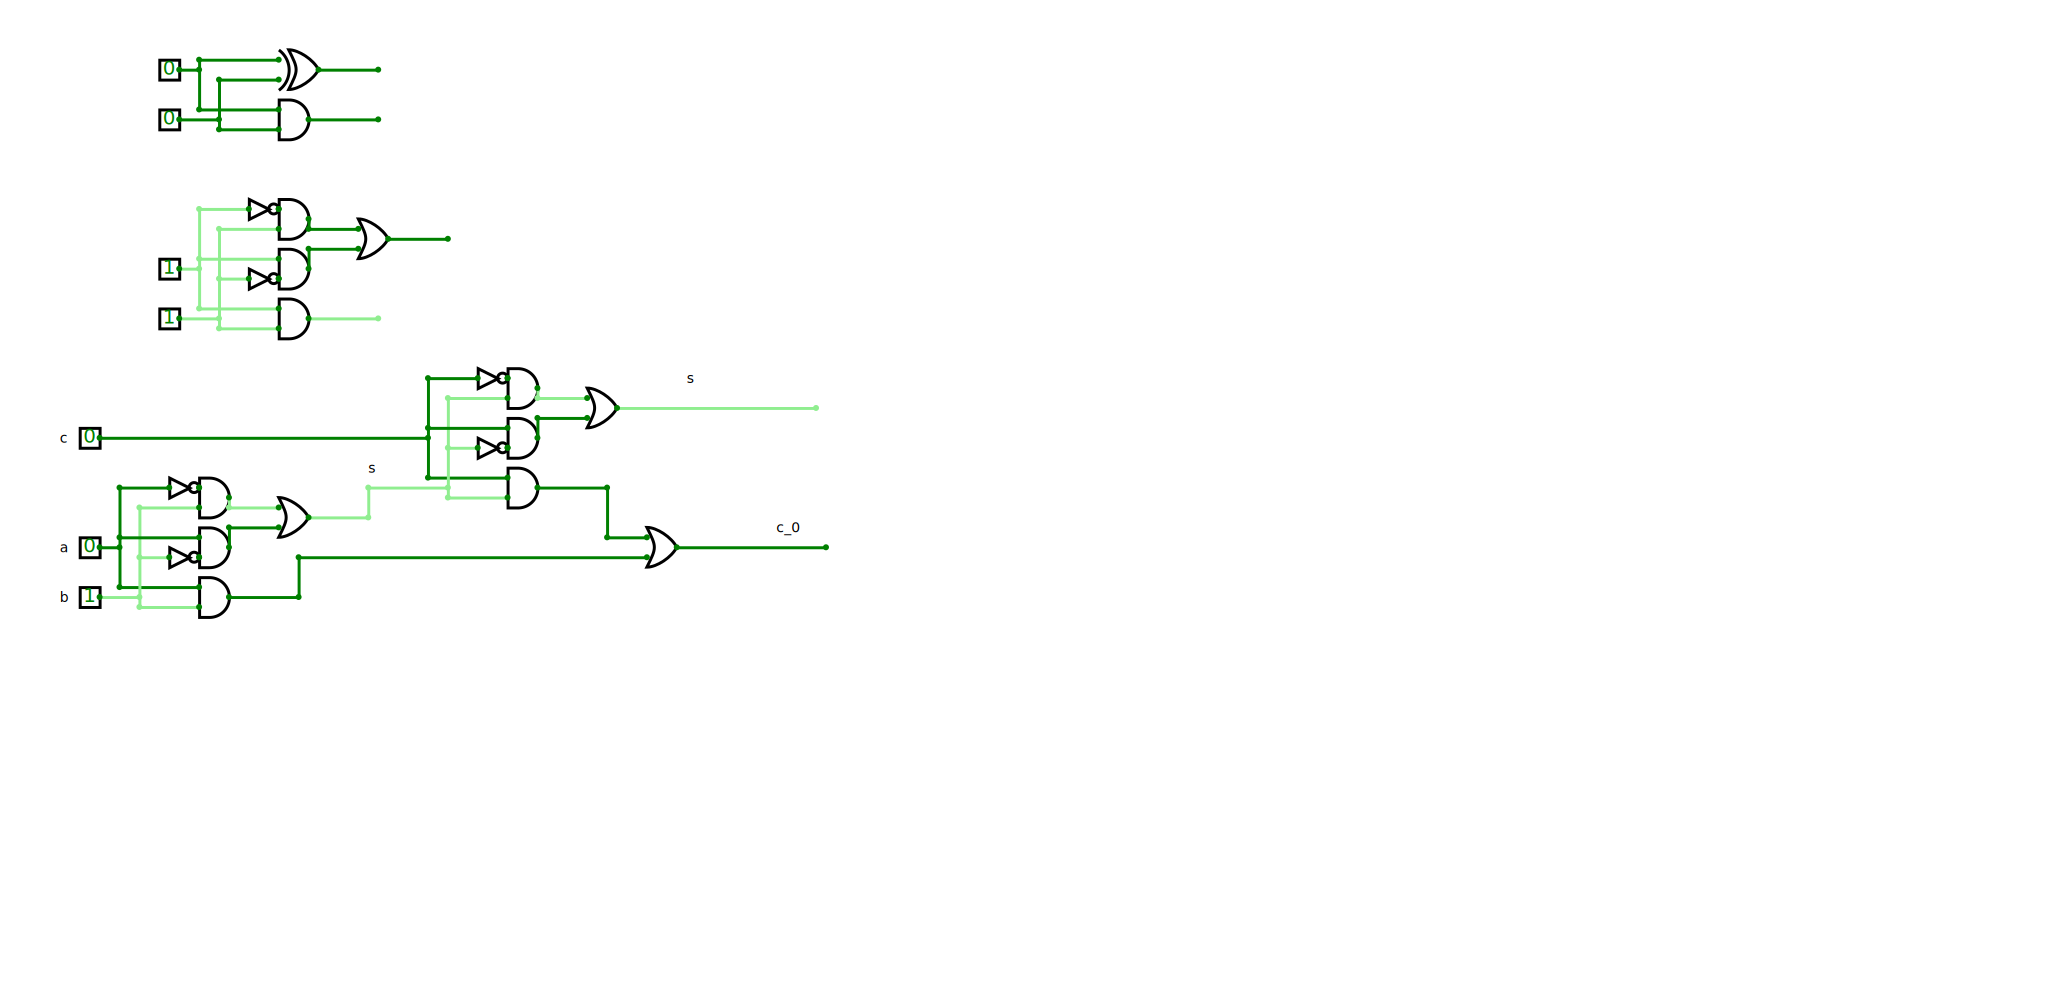
\includegraphics[scale=0.3]{./L03Z01czIII.png}
\end{center}
koniec zabawy,\\
$c_0=bc+ab+ac = (abc) + (\bar abc) +ab + abc + (\bar bac) = ab(1 + c + c) + (\bar abc) +(\bar bac) = ab + \bar{a}bc + \bar{b}ac $\\
a odczytując z bramek logicznych z wykładu mamy:\\
$c_0 = ab + \bar{a}bc + \bar{b}ac $\\
Czyli to jest równoważne. Kolej na s:\\
$s=a\bar{b}\bar{c} + \bar{a}\bar{b}c + abc + \bar{a}b\bar{c}=a\bar{b}\bar{c}+ \bar{a}b\bar{c} + \bar{a}\bar{b}c + abc = \bar{c}(a\bar{b}+ \bar{a}b)+ c(\bar{a}\bar{b} + ab) = \bar{c}(a\bar{b}+ \bar{a}b)+ c(\neg(a+b) +\neg(\bar{a}+\bar{b}))=\bar{c}(a\bar{b}+ \bar{a}b)+ c\neg((a+b)(\bar{a}+\bar{b}))=\bar c(\bar{a}b + \bar{b}a) + \neg(\bar{a}b + \bar{b}a)c$\\
co jest ponownie równoważne:\\
$s=\bar c(\bar{a}b + \bar{b}a) + \neg(\bar{a}b + \bar{b}a)c$
\section{Udowodnij, że przy sumowaniu liczb binarnych prawdziwa jest zależność $c_k = a_k \oplus b_k \oplus s_k$. (Oznaczenia są zgodne z wykładem.)}
wiemy że operacja xorowania jest przemienna, z tego też powodu rozpatrzę dwa przypadki.
\begin{enumerate}
	\item $a_k \oplus b_k = 0$\\
	skoro tak to $c_k = 0 \oplus s_k = s_k$. I rzeczywiście, w przypadku gdy suma dwóch bitów przy dodawaniu wynosi zero to bit wynikowy jest zależny od bitu przenoszonego.
	\item $a_k \oplus b_k = 1$\\
	skoro tak to $c_k = 1 \oplus s_k $. W przypadku kiedy bit sumy jest równy 1, to znaczy, że bit przenoszenia musi być równy 0.\\
	analogicznie jeżeli bit sumy jest równy 0, to bit przenoszenia musi być równy 1, aby przeniósł bit który wynikł z sumy.
	\section{Udowodnij poznaną na wykładzie zależność, że przy sumowaniu liczb binarnych w kodzie uzupełnień do dwóch występuje przepełnienie wtedy i tylko wtedy, gdy dwa ostatnie bity przeniesienia (dla znaku oraz wyjściowy) są różnych znaków. Innymi słowy, pokaż, że:\\ $$a_{n-1}= b_{n-1} = \bar s_{n-1} \Leftrightarrow c_{n-1} = \bar{c}_n$$}
	\textbf{kod uzupełnień do dwóch} to reprezentacja liczby -n w postaci $2^k - n$
	temu też przepełnienie bardzo łatwo wyłapać, przepełnienie dla sumowania występuje wyłącznie wtedy, gdy podczas operacji dodawania liczb z tym samym znakiem zmienia się znak.
	\begin{enumerate}
	\item $a_{n-1}= b_{n-1} = \bar s_{n-1} \Rightarrow c_{n-1} = \bar{c}_n$\\
	niech $a_{n-1}= b_{n-1} = \bar s_{n-1} = 1$. skoro tak to po zsumowaniu $a_{n-1}$ i $b_{n-1}$ $s_{n-1} = 0$, w takim przypadku $c_{n-1} = 0$ (ponieważ $s_{n-1} = 0$) a $c_{n}$ wyniesie 1 (ponieważ $a_{n-1}=b_{n-1}=1$).\\
	niech $a_{n-1}= b_{n-1} = \bar s_{n-1} = 0$. skoro tak to po zsumowaniu $a_{n-1}$ i $b_{n-1}$ $s_{n-1} = 1$, w takim przypadku $c_{n-1} = 1$ (ponieważ $s_{n-1} = 1$) a $c_{n}$ wyniesie 0 (ponieważ $a_{n-1}=b_{n-1}=0$).\\
	\item $a_{n-1}= b_{n-1} = \bar s_{n-1} \Leftarrow c_{n-1} = \bar{c}_n$\\
	niech $c_{n-1} = \bar{c}_n = 1$, skoro tak, to aby uzyskać podaną własność, to $a_{n-1} = 0, b_{n-1} = 0, s_{n-1} = 1$ co zgadza się z pierwszym równaniem\\
	niech $c_{n-1} = \bar{c}_n = 0$, skoro tak, to aby uzyskać podaną własność, to $a_{n-1} = 1, b_{n-1} = 1, s_{n-1} = 0$ co zgadza się z drugim równaniem\\
	oczywiście do drugiej części można skomponować więcej przykładów, dla których $a_{n-1} \neq b_{n-1}$, ale pierwszy punkt ogranicza nam zakres przypadków, (logika dla informatyków)
	\section{Określ, ile bramek potrzeba, aby zaimplementować ośmiobitowy sumator z przewidywaniem przeniesienia, jeśli możemy używać bramek o co najwyżej czterech wejściach.}
	\begin{center}
\includegraphics[scale=0.2]{./L03Z04.png}
	\end{center}
	dla 8 bitów trzeba przygotować odpowiednie $g_i$ i $p_i$
	czyli wstępnie mamy 16 bramek, do tego należy dodać kolejne 8 do wyliczenia sumy, 24.
	Pozostaje obliczyć liczbę bramek dla $c_i$.
	dla każdego z nich będziemy potrzebowali $i$ bramek and, czyli $1+2+3+5+7+9+12+15= 54$, mamy 78 bramek. Na koniec pozostały bramki or, dla $c_1,c_2,c_3$ mamy po 1 bramce (sumarycznie 3), $c_4, , c_5, c_6$ po 2 bramkach, a $c_7, c_8$ będzie miał 3. 78+3+6+6 = 93
	\section{Narysuj kompletny schemat sumatora hierarchicznego dla liczb czterobitowych zbudowanego z dwóch bloków dwubitowych.}
	\begin{center}
	\includegraphics[scale=0.075]{./L03Z05.jpg}
	\end{center}
	\section{Wskaż ścieżkę krytyczną układu mnożącego z wykładu. Podaj, jak długa (w bramkach) jest ta ścieżka.}
	Ścieżka krytyczna, to najdłuższa ścieżka w układzie cyfrowym.
	W zadaniu jest 12, ponieważ przenoszenia w poziomie Full Addera wynosi 2, a w pionie 1
	\begin{center}
	\includegraphics[scale=0.5]{./L03Z06.png}
	\end{center}
	\section{Podaj, z jakich powodów projektant układu mógłby zdecydować się na użycie sumatora szeregowego zamiast sumatora wykorzystującego przewidywanie przeniesienia.}
	w momencie kiedy mamy ograniczenia fizyczne, typu mała liczba bramek, albo potrzebujemy prostsze w budowie.
	\section{Zaprojektuj obwód obliczający uzupełnienie do 9 cyfry BCD (czyli wartość 9 - d). Zachowanie układu dla wartości 10-15 (nie odpowiadających cyfrom BCD) mogą być dowolne.}
	\textbf{BCD} to inaczej binary coded decimal
	\begin{center}
	\includegraphics[scale=0.075]{./L03Z08.png}
	\end{center}
	\section{Zaprojektuj układ wyświetlający cyfrę BCD na wyświetlaczu 7-segmentowym}
	zróbmy tabelkę:
	\begin{center}
	\begin{tabular}{|c|c|c|c||c|c|c|c|c|c|c|c|} 
	 \hline
	$A$ & $B$ & $C$ & $D$ & $a$ & $b$ & $c$ & $d$ & $e$ & $f$ & $g$ \\ 
	 \hline \hline
	 0&0&0&0& 1&1&1&1&1&1&0\\ \hline
	 0&0&0&1& 0&1&1&0&0&0&0\\ \hline
	 0&0&1&0& 1&1&0&1&1&0&1\\ \hline
	 0&0&1&1& 1&1&1&1&0&0&1\\ \hline
	 0&1&0&0& 0&1&1&0&0&1&1\\ \hline	 
	 0&1&0&1& 1&0&1&1&0&1&1\\ \hline
	 0&1&1&0& 1&0&1&1&1&1&1\\ \hline
	 0&1&1&1& 1&1&1&0&0&0&0\\ \hline
	 1&0&0&0& 1&1&1&1&1&1&1\\ \hline
	 1&0&0&1& 1&1&1&1&0&1&1\\ \hline
	\end{tabular}\\
	\begin{tabular}{|c|c|c|c|c|} 
	 \hline
	AB\textbackslash CD& 00 & 01 & 11 & 10\\  \hline
	 				 00&1&0&1&1\\ \hline
	 				 01&0&1&1&1\\ \hline
	 				 11&X&X&X&X\\ \hline
	 				 10&1&1&X&X\\ \hline
	
	\end{tabular}\\
	$$a= \bar{B}\bar{D} + C + BD + A$$
	\begin{tabular}{|c|c|c|c|c|} 
	 \hline
	AB\textbackslash CD& 00 & 01 & 11 & 10\\  \hline
	 				 00&1&1&1&1\\ \hline
	 				 01&1&0&1&0\\ \hline
	 				 11&X&X&X&X\\ \hline
	 				 10&1&1&X&X\\ \hline
	\end{tabular}\\
	$$b= \bar{B} + \bar{C}\bar{D} + CD$$
	\begin{tabular}{|c|c|c|c|c|} 
	 \hline
	AB\textbackslash CD& 00 & 01 & 11 & 10\\  \hline
	 				 00&1&1&1&0\\ \hline
	 				 01&1&1&1&1\\ \hline
	 				 11&X&X&X&X\\ \hline
	 				 10&1&1&X&X\\ \hline
	
	\end{tabular}\\
	$$c= \bar{C} + D + B$$
	\begin{tabular}{|c|c|c|c|c|} 
	 \hline
	AB\textbackslash CD& 00 & 01 & 11 & 10\\  \hline
	 				 00&1&0&1&1\\ \hline
	 				 01&0&1&0&1\\ \hline
	 				 11&X&X&X&X\\ \hline
	 				 10&1&1&X&X\\ \hline

	\end{tabular}\\
	$$d = \bar{B} \bar{D} + \bar{B}C + B\bar{C}D + C\bar{D} + A$$
	\begin{tabular}{|c|c|c|c|c|} 
	 \hline
	AB\textbackslash CD& 00 & 01 & 11 & 10\\  \hline
	 				 00&1&0&0&1\\ \hline
	 				 01&0&0&0&1\\ \hline
	 				 11&X&X&X&X\\ \hline
	 				 10&1&0&X&X\\ \hline
	
	\end{tabular}\\
	$$ e = \bar{B}\bar{D} + C \bar{D}$$
	\begin{tabular}{|c|c|c|c|c|} 
	 \hline
	AB\textbackslash CD& 00 & 01 & 11 & 10\\  \hline
	 				 00&1&0&0&0\\ \hline
	 				 01&1&1&0&1\\ \hline
	 				 11&X&X&X&X\\ \hline
	 				 10&1&1&X&X\\ \hline
	
	\end{tabular}\\	
	$$f = \bar{C}\bar{D} + B \bar{C} + B\bar{D} + A$$	
	\begin{tabular}{|c|c|c|c|c|} 
	 \hline
	AB\textbackslash CD& 00 & 01 & 11 & 10\\  \hline
	 				 00&0&0&1&1\\ \hline
	 				 01&1&1&0&1\\ \hline
	 				 11&X&X&X&X\\ \hline
	 				 10&1&1&X&X\\ \hline
	\end{tabular}\\
	$$g = \bar{B}C + B\bar{C} + A + B\bar{D}$$
	\end{center}
	teraz należy napisać układ który spełni nam wszystkie zapisane tutaj zależności
	\section{Jaki przedział wartości może być reprezentowany przez liczby stałoprzecinkowe o następujących formatach:}
	\begin{enumerate}
		\item 24-bitowe liczby stałoprzecinkowe bez znaku z 12 bitami części ułamkowej,\\
		minimalnie 0, maksymalnie $2^{12}-1 + 1 - \frac{1}{2^{12}}$
		\item 24-bitowe liczby stałoprzecinkowe ze znakiem w kodzie znak-moduł z 12 bitami części ułamkowej,\\
		minimalnie $-2^{11} +  \frac{1}{2^{12}}$, maksymalnie $2^{11} - \frac{1}{2^{12}}$
		\item 24-bitowe liczby stałoprzecinkowe ze znakiem w kodzie uzupełnień do dwóch z 12 bitami części
ułamkowej.\\
przyjąłem że U-2 przenosi się do końca
minimalnie $-2^{11}$, maksymalnie $2^{11} - \frac{1}{2^{12}}$
	\end{enumerate}
	
%1 1 1 1 1  1  1  1   1   1   1    1
%1 2 4 8 16 32 64 128 256 512 1024 2048 
\end{enumerate}
	
\end{enumerate}
\end{document}